%!TEX root = Manuscrit.tex
\chapter{Extension aux capteurs non-conventionnels}
\label{chap:extension}
%\citationChap{I suppose it is tempting, if the only tool you have is a hammer, to treat everything as if it were a nail.}{Abraham Maslow}
\minitoc

\chapsummary{%
  Les images multispectrales peuvent être traitées par des réseaux type SegNet de la même façon que les images usuelles. Toutefois, il n'est pas possible de faire de l'apprentissage par transfert et du pré-entraînement compte-tenu de la différence de nombre de bandes. En pratique, les expériences montrent que trois bandes suffisent à obtenir des résultats équivalents. Utiliser quatre bandes IRRVB ne semble pas apporter de gain et dégrade même légèrement les performances compte-tenu de l'absence de pré-entraînement.

  Travailler sur les modèles numériques de terrain se fait bien et sans trop de problème, si ce n'est l'absence d'information. On les traite comme des images en niveaux de gris et cela se passe bien.

  Travailler sur les images hyperspectrales demande d'être soigneux et de faire attention à ce que l'on fait, mais dans l'ensemble la litérature propose des solutions pertinentes.
}

\newpage

\section{Images multispectrales}

\subsection{Prise en compte du proche infrarouge}

Les images multispectrales les plus simples sont des images à trois ou quatre canaux comprenant un canal infrarouge. En l'occurrence, les jeux de données \gls{ISPRS} Vaihingen et Potsdam comportent de telles données multispectrales, respectivement \gls{IRRV} et \gls{IRRVB}.

Dans le chapitre précédent, nous avons montré qu'il était possible et de traiter les images \gls{IRRV} de la même façon que les images \gls{RVB} traditionnelles. En particulier, cela nous a permis de transférer les poids de réseaux de pré-entraînés sur ImageNet à des images de télédétection \gls{IRRV}. Toutefois, dans le cas des images multispectrales \gls{IRRVB}, il est impossible de réaliser ce transfert en conservant les quatre canaux. Notre approche précédente a consisté à utiliser seulement les trois canaux \gls{RVB}, en omettant le canal infrarouge.

Nous réalisons une étude préliminaire sur le jeu de données \gls{ISPRS} Potsdam en reprenant les modèles et hyperparamètres obtenus dans le~\cref{chap:cartographie}. En particulier, nous étudions différentes variantes de SegNet, avec et sans initialisation de l'encodeur à partir des poids de VGG-16 pré-entraîné sur ImageNet, sur différentes combinaisons de canaux. Les résultats sont détaillés dans le~\cref{tab:comparaison_bandes}. Les tuiles 2\_11, 7\_10, 4\_10, 7\_9, 7\_12, 6\_8, 6\_7, 6\_9, 5\_11, 2\_10, 2\_12, 3\_10, 6\_10, 6\_11, 3\_12, 3\_11, 5\_12 et 4\_12 sont utilisées pour l'entraînement tandis que la validation s'effectue sur les tuiles 4\_11, 6\_12, 7\_11, 5\_10, 7\_8 et 7\_7.

\begin{table}
  \setlength\tabcolsep{3pt}
  \caption{Comparaison des résultats obtenus par SegNet sur Potsdam à partir de plusieurs combinaisons de canaux.}
  \label{tab:comparaison_bandes}
  \begin{tabularx}{\textwidth}{Y Y c c c c c c c}
    \toprule
    Canaux & Pré-entraînement & Routes & Bâtiments & Arbres & Vég. basse & Véhicules & Autres & Exactitude\\
    \midrule
    IR+B & n & 72.79 & 87.22 & 57.61 & 71.74 & 87.05 & 13.15 & 70.69\\
    R+G & n & 89.92 & 95.80 & 81.49 & 84.30 & 95.21 & 40.42 & 88.48\\
    IR+R & n & 90.75 & 95.89 & 82.77 & 84.97 & 95.50 & 42.47 & 89.25\\
    \glsname{IRRV} & n & 90.83 & 95.91 & 83.31 & 84.26 & 94.99 & 43.74 & 89.29\\
    \glsname{RVB} & n & 90.40 & 96.32 & 82.38 & 83.78 & 95.42 & 39.97 & 89.02\\
    \glsname{IRRVB} & n & 89.67 & 95.57 & 82.35 & 83.82 & 95.17 & 42.89 & 88.51\\
    \glsname{RVB} & o & 92.35 & \textbf{97.62} & 85.18 & 87.19 & \textbf{96.11} & \textbf{52.15} & 91.22\\
    \glsname{IRRV} & o & \textbf{92.51} & 97.34 & \textbf{85.68} & \textbf{87.54} & \textbf{96.11} & 50.24 & \textbf{91.28}\\
    \bottomrule
  \end{tabularx}
\end{table}

Ces expériences préliminaires montrent que les résultats obtenus à l'aide des trois canaux \gls{RVB} et \gls{IRRV} sont très similaires sur Potsdam. Cependant, les modèles n'utilisant que trois canaux sont légèrement plus exacts que les modèles à quatre canaux \gls{IRRVB}, même lorsqu'ils sont initialisés aléatoirement, c'est-à-dire sans pré-entraînement. En particulier, les résultats à partir des combinaisons de 2 canaux semblent indiquer que l'interaction entre les canaux infrarouge et bleu entraîne une baisse conséquente des performances du modèle à cause d'une confusion considérable entre la classe "autres" et les autres classes. Cette chute des performances apparaît y compris lorsque le réseau n'apprend pas sur les pixels appartenant à la classe "autres", c'est-à-dire que l'interaction des canaux infrarouge et bleu introduit bien une confusion que SegNet ne parvient pas à contourner.

\todo[inline]{Corrélations entre bandes, résultats avec ResNet}

\subsection{Images multispectrales}

La plupart des capteurs optiques embarqués dans des satellites d'observation de la Terre réalisent des acquisitions multispectrales. Dans ce cas, les bandes ne sont pas nécessairement toutes de même largeur, ni restreintes aux longueurs d'ondes du domaine visible. Nous nous intéressons donc à l'utilisation des modèles de type SegNet pour la segmentation sémantique d'images satellites multispectrales.
En particulier, nous bénéficions d'un jeu de données d'images Sentinel-2 accompagnées de la carte d'occupation du sol GlobeCover 2009. Les images Sentinel-2 considérées couvrent une région se situant à la frontière de la France, de la Suisse et de l'Italie. Les images ont été acquises entre mai et octobre 2016.

Un premier jeu de données est composé des images ne contenant aucune couverture nuageuse (nuages opaques ou cirrus). Un second jeu de données est constitué uniquement sur la période d'été mais inclut également les tuiles comprenant une couverture nuageuse, dont la détection est désormais prise en compte dans la tâche de classification. Les deux jeux de données sont ainsi constituées d'acquisitions sur les mêmes zones à plusieurs dates. Les images Sentinel-2 sont interpolées à une résolution de \SI{20}{\meter/\px} pour toutes les bandes tandis que les annotations issues de GlobeCover sont à une résolution de \SI{300}{\meter/\px}. Les détails des jeux de données sont indiqués dans le~\cref{tab:datasets}.

\begin{table}
\caption{Deux jeux de données d'images Sentinel-2 sont considérés. Le premier s'étend sur une longue période mais exclut les images contenant une couverture nuageuse. Le second est restreint à une période temporelle plus courte mais inclut les images en présence de nuages. Les deux jeux de données contiennent environ 150 millions de pixels chacun.}
\label{tab:datasets}
\begin{tabular}{lccc}
\toprule
Jeux de données & \multicolumn{3}{c}{nombre d'images}\\
(période)  & entraînement & validation  & nombre de classes \\
\midrule
D1, période longue sans nuages & & & \\
 (mai--oct. 2016) & 140 & 54 & 23 \\
\midrule
D2, période courte avec nuages & & & \\
(juin--août 2016) & 158 & 39 & 24 \\
\bottomrule
\end{tabular}
\end{table}

L'ensembles des 13 bandes de Sentinel-2 sont fournis au entrée au réseau. Nous coupons la fin du décodeur de SegNet, car il ne nous est pas utile d'obtenir des cartes à résolution $1:1$. Nous réalisons simplement des cartes à échelle $1:8$ (\SI{160}{\meter/\px}) ce qui diminue le nombre de paramètres à optimiser et le temps de calcul, puis nous interpolons les cartes de probabilités à résolution \SI{300}{\meter/\px} avant le calcul du \emph{softmax}.



\todo[inline]{article avec A. Benoit}
\todo[inline]{collab ESA}

\section{Imagerie hyperspectrale}

\begin{figure}
  \begin{minipage}[t]{0.485\textwidth}
      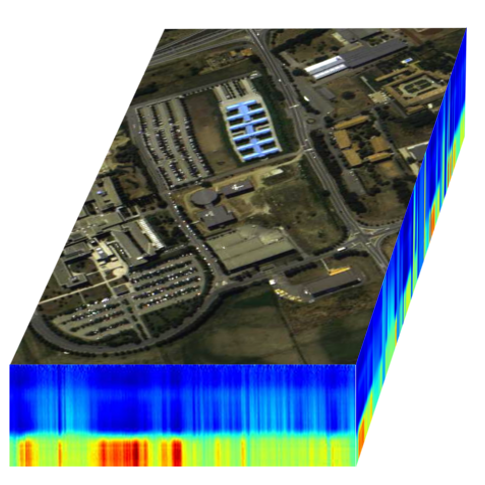
\includegraphics[width=\textwidth]{hyperspectral_cube_pavia}
      \caption{Exemple de cube hyperspectral sur le jeu de données \emph{Pavia University}.}
      \label{fig:cube_hyperspectral}
  \end{minipage}
  \hfill
  \begin{minipage}[t]{0.485\textwidth}
      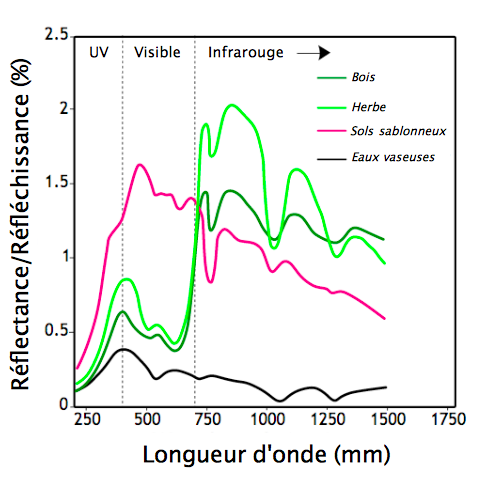
\includegraphics[width=\textwidth]{reflectances}
      \caption{Exemple de réflectances caractéristiques de diverses surfaces terrestres.}
      \small{Crédits image\,: \href{https://commons.wikimedia.org/wiki/File:R\%C3\%A9flectance_surfaces_terrestres.png}{Arbeck (Wikimedia Commons, CC-BY-SA 3.0)}}
      \label{fig:reflectances}
  \end{minipage}
\end{figure}

Grâce aux avancées en apprentissage profond pour le traitement d'images et la reconnaissance de formes, la classification d'images de télédétection a effectué d'importants progrès en quelques années. En particulier, l'imagerie optique traditionnelle (\gls{RVB} et infrarouge) a fortement bénéficié de l'utilisation des réseaux de neurones convolutifs profonds pour les tâches de classification, de détection d'objets et de segmentation sémantique~\cite{audebert_semantic_2016,volpi_dense_2017,marmanis_semantic_2016}. Cependant, la vision par ordinateur traditionnelle se borne à manipuler des images encodées sur trois canaux au format Rouge-Vert-Bleu (RVB), voire en niveaux de gris. Or, la télédétection s'appuie bien souvent sur l'imagerie multispectrale (satellites Sentinel-2, AVIRIS, Landsat\dots), permettant d'acquérir simultanément les réponses lumineuses sur plusieurs bandes de longueurs d'onde. Les acquisitions hyperspectrales forment sous-ensemble de l'imagerie multispectrale pour lequel le nombre de bandes spectrales est particulièrement élevé, permettant une analyse fine des sols et des matériaux~\cite{cubero-castan_physics-based_2015,fabre_estimation_2015}.

En effet, les capteurs en hyperspectral disposent d'une faible résolution spatiale, mais d'une très grande résolution spectrale et mesurent de fait la réponse lumineuse d'un objet sur plusieurs centaines de bandes de fréquences. Les méthodes purement orientée vision de \textit{deep learning} ne se transposent pas trivialement au cube de données hyperspectrales, car la dimension spectrale prédomine devant les dimensions significatives du voisinage spatial dans la plupart des situations. Une acquisition typique en aérien aura une résolution au sol au mieux de 1m/pixel mais une résolution spectrale d'environ 10nm/bande sur 200 bandes entre 0,4µm et 2,5µm. Une maison de $12m\times10m$ ($120m^2$, la moyenne en France) sera donc décrite par un tenseur de taille $12\times10\times200$ ! En comparaison, une caméra optique permet d'obtenir des acquisitions à une résolution de l'ordre de 10cm/px en RVB sur 3 bandes entre 0,4µm et 0,7µm (domaine visible), soit un tenseur de taille $120\times100\times3$. La quantité de données est similaire (24 000 scalaires contre 36 000), mais leur répartition est nettement différente. En pratique, on parle ainsi de cube hyperspectral, car la dimension spectrale possède un poids équivalent à celle des dimensions spatiales, comme illustré par la~\cref{fig:cube_hyperspectral}. En outre, la faible résolution spatiale des capteurs hyperspectraux va également être un facteur limitant dans le nombre d'échantillons annotés disponibles pour l'entraînement de modèles statistiques. Dans la pratique, une acquisition hyperspectrale aérienne ou satellite résultera en des images plus petites à couverture égale par rapport à l'imagerie optique. Ces deux points sont les principaux défis à relever pour utiliser l'apprentissage profond dans le cadre du traitement d'images hyperspectrales.

Ce document rappelle en premier lieu les principes de l'imagerie hyperspectrale afin de mettre en évidence les différence par rapport aux images RVB traditionnelles et brossera un portrait des jeux de données disponibles publiquement. Nous verrons ensuite quelles approches d'apprentissage classique sont utilisées pour classifier ces données, avant de s'intéresser plus prêt aux travaux récents utilisant l'apprentissage profond et d'évoquer plusieurs pistes de travail potentielles.

\subsection{Principes physiques de l'imagerie hyperspectrale}
%\textit{Paragraphe rédigé à partir d'éléments d'un mail de Xavier Ceamanos, ONERA.}

Physiquement, un capteur hyperspectral mesure\footnote{Après une phase d'étalonnage.} l'intensité (en unité de luminance spectrale) du flux lumineux par unité de surface et par unité d'angle solide. Il s'agit d'une grandeur physique qui a pour unité le $W.m^{-2}.str^{-1}$. Ce flux lumineux est mesuré par le capteur pour différentes bandes radiométriques, dont la largeur est de l'ordre d'une dizaine de nanomètres. Ainsi, pour chaque unité de surface (qui se traduira par un pixel dans l'image finale), le capteur acquiert un spectre discret de plusieurs centaines de bandes. Chacun de ces spectres peut se représenter sous la forme d'une courbe de réponse spectrale, comme illustré par l'histogramme de la~\cref{{fig:reflectances}}. Il est important de noter que les différentes composantes de ce flux lumineux intègrent aussi bien la lumière émise et réfléchie par l'objet que celle provenant de l'environnement, qui s'ajoutent à la mesure.

Notamment, dans le cadre de la télédétection pour l'observation de la Terre, les acquisitions sont réalisées depuis le sommet de l'atmosphère (en satellite) ou depuis l'atmosphère même (en aéroporté). Le signal provenant de la surface est ainsi altéré par les perturbations atmosphériques. Par exemple, une image hyperspectrale de télédétection permet d'observer les surfaces, mais aussi les nuages, les effets de brumes, les aérosols en suspension dans l'air, etc. Or, la majorité des applications\footnote{Du moins, celles qui nous intéressent en observation de la Terre.} concernent l'analyse des surfaces et des matériaux au sol. On s'intéresse donc plutôt à la réflectance du matériau, définie comme le rapport entre le flux émis par une surface et le flux incident~:
$$\rho = \frac{\phi_{r\acute{e}fl\acute{e}chi}}{\phi_{incident}}$$
Ce rapport indique le pouvoir réfléchissant d'un objet vis-à-vis d'une certaine longueur d'onde lumineuse (on parle également d'albédo du matériau). C'est une grandeur sans unité comprise entre 0 (surface complètement absorbante) et 1 (surface totalement réfléchissante). En règle générale, un matériau renvoyant plus de 80\% de la lumière blanche apparaît blanc, tandis qu'un matériau réfléchissant moins de 3\% apparaît noir. Dans le cas de la réflectance radiométrique, cet indice est mesuré pour chaque bande de fréquences du capteur, ce qui permet de dessiner un histogramme des réflectances en fonction de la longueur d'onde lumineuse. L'avantage majeur de la réflectance est d'être une propriété intrinsèque des matériaux, indépendante de l'environnement extérieur, et dotée d'un fort pouvoir discriminant~\cref{fig:reflectances}. De fait, on obtient généralement de meilleurs résultats à partir de ces données corrigées en réflectance.

\paragraph{Corrections environnementales}
Les physiciens cherchent à compenser les phénomènes perturbatoires par des méthodes dites de correction atmosphérique~\cite{deschamps_atmospheric_1980, rahman_smac:_1994, chavez_image-based_1996} afin de se débarrasser de l'influence de l'atmosphère et d'obtenir une grandeur permettant de caractériser le type de sol~\cite{gao_atmospheric_2009}. Celles-ci prennent des images en luminance en entrée et produisent des images en unité de réflectance de surface. La correction atmosphérique permet d'obtenir la réflectance en rendant négligeable l'influence de la diffusion lumineuse et des phénomènes radiatifs dans l'atmosphère. Cette correction s'effectue en utilisant des modèles physiques estimant les effets radiatifs et les perturbations atmosphériques en fonction de plusieurs paramètres physiques. Généralement, cela implique d'avoir accès à des informations météorologiques, en particulier l'ensoleillement. Ceci peut-être obtenu a posteriori grâce aux éphémérides ou, dans certains cas en aéroporté (avion ou drone), grâce à un capteur d'ensoleillement embarqué sur le dos de l'appareil mesurant en temps réel les conditions d'illumination. À noter que pour un capteur hyperspectral ``à main'', celui-ci illumine directement la cible de la mesure via un éclairage actif, permettant ainsi de s'affranchir de ces conditions environnementales.
Par ailleurs, il est important de noter que le calcul du flux réfléchi se fait généralement sous hypothèse de planarité du sol. En effet, si le sol n'est pas plan, alors les réflexions peuvent être complexes à modéliser et des phénomènes d'ombrage ou de sur-illumination apparaissent (on parle de réflexions multiples). Il est donc parfois nécessaire d'utiliser un modèle de surface pour corriger les données, notamment en milieu urbain~\cite{ceamanos_using_2017}.
Enfin, il faut garder à l'esprit que ce type de corrections, atmosphérique ou de terrain, peuvent elles aussi introduire des erreurs et des incertitudes dans les données, bien qu'il s'agisse d'une pratique courante et relativement bien maîtrisée.

\paragraph{Visualisation}
Contrairement à la vision humaine, l'imagerie hyperspectrale capte la réponse spectrale d'une surface sur de nombreuses bandes de fréquences (et pas seulement rouge, vert et bleu). La résolution spectrale est ainsi nettement plus fine et la plage d'acquisition s'étend au-delà du spectre du visible, comprenant plusieurs centaines de bandes d'environ 10nm de large sur un domaine pouvant aller de l'ultra-violet (\SI{300}{\nano\meter}) jusqu'à la limite de l'infrarouge moyen (\SI{3 000}{\nano\meter}). En comparaison, le spectre visible ne couvre que les longueurs d'onde de \SI{300}{\nano\meter} à $\simeq$ \SI{700}{\nano\meter}. Traditionnellement, on visualise une image optique \gls{RVB} comme l'agrégation de trois cartes d'intensité en rouge, vert et bleu. En revanche, dans le cas d'une image hyperspectrale, il est plus pertinent de se représenter la donnée comme un cube dont deux dimensions représentent l'espace tandis que la troisième correspond aux intensités spectrales. Chaque pixel contient la réponse spectrale complète du point observé. Ces signatures spectrales caractérisent les surfaces et les matériaux lorsqu'ils sont purs. En pratique, la faible résolution spatiale implique bien souvent qu'une surface atomique d'acquisition recouvre plusieurs matériaux, le spectre mesuré étant alors un mélange. Par ailleurs, les classes d'intérêt en télédétection présentent de toute façon une propension naturelle à se mélanger avec d'autres éléments (mélanges de végétations éparses, sables bitumineux\dots).

Toutefois, compte-tenu de la différence des résolutions spectrales entre l'hyperspectral (très petite devant celle des yeux humains) et de l'imagerie \gls{RVB} classique, il n'y a pas d'équivalence entre les deux représentations. Ainsi, une image hyperspectrale contient bien plus d'information que l'image \gls{RVB} \emph{à résolution spatiale identique}. En outre, s'il est possible de reconstruire une image \gls{RVB} composite à partir de bandes spectrales bien choisies dans l'image hyperspectrale, les différences de résolution font qu'il ne s'agit que d'une pseudo-image, qui n'aurait pas été vue de cette façon par des yeux humains. En effet, un appareil photo fonctionne en captant séparément la lumière rouge, verte et bleue grâce à un filtre, de façon à simuler le fonctionnement de l'\oe{}il humain. Un capteur hyperspectral fera généralement une acquisition ligne par ligne du spectre complet, décomposé par un prisme (capteur dit ``\textit{pushbroom}''). Les deux modes d'acquisition ne sont ainsi pas comparables.

\subsection{Jeux de données}

La communauté scientifique dispose de plusieurs jeux de données publics utilisant un capteur hyperspectral ainsi que des annotations permettant d'évaluer des performances de classification\footnote{\url{http://www.ehu.eus/ccwintco/index.php?title=Hyperspectral_Remote_Sensing_Scenes}}. Nous présentons ici les plus utilisés, par autre de popularité.

\subsubsection{Pavia}

La principale difficulté des approches par apprentissage statistique sur des données hyperspectrales réside dans le faible nombre d'échantillons disponibles. En effet, dû aux différences de capteurs, de conditions d'exposition et d'étalonnage, il est difficile d'exploiter conjointement plusieurs jeux de données. Or, individuellement, les images hyperspectrales annotées mises à disposition de la communauté scientifique sont de taille très faible en comparaison des banques d'images RVB traditionnelles. Cela rend difficile l'évaluation des méthodes d'apprentissage supervisées et ne permet que rarement d'exploiter au mieux les modèles de \textit{deep learning}. Les images acquises par le capteur AVIRIS sur le territoire américain sont disponibles en accès libre\footnote{\url{https://aviris.jpl.nasa.gov/alt_locator/}}, mais sans annotation.

Pavia est un jeu de données acquis via le capteur ROSIS avec une résolution au sol de 1,3m sur la ville de Pavie, en Italie. Il est divisé en deux scènes\,: Pavia University (103 bandes, $610\times340$px) et Pavia Centre (102 bandes, $1096\times715$px). 9 classes d'intérêt sont annotées, couvrant différents matériaux urbains (brique, asphalte, métaux), l'eau et la végétation sur 50\% de la surface capturée.

Il s'agit d'un des principaux jeux de données de référence dans la communauté, notamment car il s'agit des plus grandes images hyperspectrales annotées disponibles. Toutefois, certains pixels de la scène ne contiennent pas d'information spectrale et doivent être éliminés. En outre, quelques erreurs se sont glissées dans la vérité-terrain.

\subsubsection{Indian Pines}

Indian Pines est un jeu de données acquis en utilisant le capteur américain AVIRIS. La scène couvre une surface agricole sur 224 bandes spectrales pour $145\times145$px, avec une résolution au sol de 3,7m/px. La majorité de l'image consiste en des champs d'une dizaine de cultures différentes, le reste étant occupé par de la végétation dense. 16 classes sont annotées, dont certaines très rares (moins de 100 échantillons). Les bandes d'absorption de l'eau (108$\rightarrow$112, 154$\rightarrow$167 et 224) sont généralement enlevées.

En dépit de sa faible taille, il s'agit d'un des principaux jeux de données de référence dans la communauté. Les classes les plus rares ne sont parfois pas prises en compte pour évaluer les algorithmes de classification.

\subsubsection{Salinas}
Salinas est un jeu de données utilisant également le capteur AVIRIS. La scène comporte $512\times217$ échantillons à 3,7m/pixel. Les bandes d'absorption de l'eau (108$\rightarrow$112, 154$\rightarrow$167 et 224) sont généralement enlevées. 16 classes sont annotées, majoritairement concernant les différentes cultures observées, la végétation et le type de sol.

\subsubsection{Kennedy Space Center (KSC)}
Le jeu de données KSC utilise le capteur AVIRIS avec une résolution au sol de 18m. Les bandes d'absorption de l'eau et celles avec un rapport signal/bruit faibles sont enlevés, pour ne conserver que les 176 bandes les plus informatives. 13 classes concernant divers types d'occupation du terrain sont annotées.

\subsubsection{Botswana}
Botswana est un jeu de données acquis sur le delta du Okavango à l'aide du senseur Hyperion embarqué par le satellite EO-1 de la NASA, à une résolution de 30m/px sur 242 bandes. Seules les 145 bandes 10$\rightarrow$55, 82$\rightarrow$97, 102$\rightarrow$119, 134$\rightarrow$164 et 187$\rightarrow$220 sont conservées, les autres correspondant aux bandes d'absorption de l'eau et à des bandes mal calibrées. 14 classes d'intérêt sont annotées concernant différents types de végétation et de marécages.

\subsubsection{NAOMI Mandji}
Le jeu de données NAOMI Mandji est une acquisition réalisée par le DOTA (ONERA Toulouse) en collaboration avec Total dans le cadre du projet de recherche NAOMI. Cette acquisition couvre les environs de Port-Gentil, sur l'île de Mandji au Gabon. La zone 2, correspondant à une image de $1944\times1196$px a été annotée sur 9 classes d'intérêt à une résolution spatiale de 1,3m/px. Au total, 416 bandes ont été acquises, 158 dans le VNIR (\textit{Visible and Near InfraRed}) et 258 dans le SWIR (\textit{Short-Wave InfraRed}). La couverture du SWIR est incluse que celle du VNIR, certains pixels n'ayant que les bandes correspondant au second.

\subsubsection{Récapitulatif}

Les caractéristiques des différents jeux de données publics identifiés sont listées dans la~\cref{tab:hyperx_datasets}. Le principal élément qui en ressort est le faible nombre d'échantillons annotés disponibles sur chacun des datasets. Le capteur AVIRIS est utilisé sur plusieurs scènes, mais les classes identifiées ne sont pas cohérentes d'une acquisition à l'autre, limitant le potentiel de réutilisation des modèles.

\begin{table}[h]
\setlength{\tabcolsep}{3pt}
\begin{tabularx}{\textwidth}{ Y c c c c c c c }
\toprule
Jeu de données & Pixels & Bandes & Domaine & Résolution & Annotations & Classes & Acquisition\\
\midrule
Pavia & 991 040 & 103 & 0,43-0,85µm & 1,3m & 50 232 & 9 & Aérienne\\
Indian Pines & 21 025 & 224 & 0,4-2,5µm & 3,7m & 10 249 & 16 & Aérienne\\
Salinas & 111 104 & 227 & 0,4-2,5µm & 3,7m & 54 129 & 16 & Aérienne\\
KSC & 314 368 & 176 & 0,4-2,5µm & 18m & 5 211 & 13 & Aérienne\\
Botswana & 377 856 & 145 & 0,4-2,5µm & 30m & 3 248 & 14 & Satellite\\
NAOMI Mandji & 1 052 012 & 416 & 0,4-2,5µm & 1,3m & 1 052 012 & 9 & Aérienne\\
\bottomrule
\end{tabularx}
\caption{Récapitulatif des principaux jeux de données publics annotés en imagerie hyperspectrale.}
\label{tab:hyperx_datasets}
\end{table}

\subsection{Approches traditionnelles}

Cette section détaille les approches traditionnelles d'analyse d'image hyperspectrale. Une attention particulière sera accordée aux méthodes d'apprentissage statistique supervisées, puisque celles-ci constituent une \textit{baseline} de référence pour les approches orientées \textit{deep learning}.

\subsubsection{Pré-traitements et normalisations}
Travailler sur des images hyperspectrales implique bien souvent d'effectuer des pré-traitements préliminaires. Outre les corrections atmosphériques et géométriques afin d'obtenir les cartes de réflectance, il est courant d'effectuer certaines opérations de normalisation des données.

\paragraph{Sélection de bandes} Selon les capteurs, il est peut arriver qu'il soit avantageux d'éliminer certaines bandes radiométriques difficiles à exploiter ou écrasant la dynamique des spectres. Les cas de figure les plus fréquents sont le rejet des bandes liées à l'absorption de l'eau, les bandes avec un faible rapport signal sur bruit et les bandes saturées.

\paragraph{Normalisation statistique}
Certaines stratégies courantes permettent de significativement améliorer la classification avec des approches statistiques. En notant $X_i$ les spectres individuels et $I$ l'image dans sa globalité, ces stratégies sont les suivantes\,:
\begin{itemize}
\item Utilisation de l'angle spectral, version normalisée du spectre avec une norme euclidienne unitaire\,:
$X = X / \| X \|$,
\item Normalisation des moments statistiques de premier et second ordres (moyenne nulle et variance unitaire), soit bande par bande, soit globalement\,:
$I = \frac{I - moy(I)}{std(I)}$,
\item Conversion numérique à une représentation dans [0, 1] par $I = \frac{I - min(I)}{max(I) - min(I)}$, soit bande par bande, soit globalement.
\end{itemize}

Afin d'éliminer l'influence des valeurs aberrantes et de rééquilibrer la dynamique numérique de l'image, il est également possible de tronquer les valeurs au-delà d'un certain seuil. Ainsi, il est courant de tronquer toutes les valeurs supérieures au 98\ieme percentile ou bien supérieure à $moy(I) + 2\times std(I)$.

\subsubsection{Classification de spectres}

L'approche la plus immédiate de l'étude de données hyperspectrales consiste à ignorer l'aspect spatial des données et de traiter l'image comme un agrégat de spectres 1D. Chaque pixel correspond alors à une signature spectrale, c'est-à-dire un signal discret sur lequel il est possible d'apprendre un modèle statistique. On se borne ici à présenter les méthodes faisant appel au \textit{machine learning} avec peu ou pas de pré-traitement expert, excepté ceux présentés précédemment.

\subsubsection{Démélange}
Dans un cadre parfait, un pixel d'une image hyperspectrale correspond à la réflectance du matériau observé sur une unité de surface. Toutefois, la résolution spatiale des images fait qu'un pixel correspond à une surface couvrant plusieurs matériaux, produisant ainsi des spectres de mélange. Concrètement, si $S_1, \dots, S_n$ désignent les spectres purs de l'ensemble des matériaux de la scène, alors en un pixel $(i,j)$, le spectre local observé sera une fonction $F$ des $S_i$ :
$$ \phi_{i,j} = F(S_1, \dots, S_n) \simeq \sum_{k = 1}^n \lambda_k S_k~.$$
Dans le cas où la surface est plane, on peut faire l'hypothèse que $F$ est une simple combinaison linéaire, où le coefficient de pondération $\lambda_k$ correspond à la proportion du matériau $k$ dans la surface observée.

Une façon de traiter l'image hyperspectrale consiste à effectuer un démélange~\cite{parra_unmixing_1999}. En effet, une façon d'obtenir une classification des matériaux présents sur la zone imagée est alors de calculer les cartes d'abondance. Les spectres de référence des matériaux purs sont appelés les \textit{endmembers}\footnote{En minéralogie, un \textit{enmember} est un minéral en bout de chaîne de pureté. La plupart des minéraux sont des solutions solides (\textit{i.e.} des mélanges de ces \textit{endmembers}).} et constituent une base de décomposition des spectres mélangés. Les cartes d'abondance correspondent aux proportions en tout pixel des différents matériaux de la zone, c'est-à-dire aux coefficients de la décomposition d'un mélange. Généralement, en connaissant les spectres purs $S_k$ et l'image $\Phi$, il est possible d'inverser le système linéaire pour obtenir les coefficients $\lambda_k$ en tout point, et donc les cartes d'abondance. Ces méthodes reposent principalement sur des mécaniques d'algèbre linéaire et des méthodes numériques d'inversion de problème. Il existe également des méthodes d'apprentissage, par exemple par \textit{clustering} permettant d'obtenir les \textit{endmembers} quand ils sont inconnus.

\subsubsection{Réduction de dimensionalité}
De nombreux travaux se sont intéressés à la réduction de la dimensionalité des spectres. En effet, compte-tenu de la résolution spectrale, les intensités voisines dans le domaine fréquentiel sont fortement corrélées. Une signature spectrale contient donc beaucoup d'information redondante, et toute la difficulté réside dans l'extraction de l'information discriminante pour diminuer le nombre de bandes pertinentes~\cite{le_bris_extraction_2015}. Ainsi, de nombreuses méthodes de pré-traitement en sélection de \textit{features} ont été utilisées, comme la génération de \textit{features} aléatoires \cite{damodaran_sparse_2017} ou encore l'analyse par composantes principales (ACP) \cite{rodarmel_principal_2002}. Cela peut également passer par le calcul d'indices physiques comme le Normalized Difference Vegetation Index (NDVI) ou le Normalized Difference Water Index (NDVWI).

La classification se fait ensuite de façon traditionnelle, en utilisant des modèles statistiques classiques : arbres de décision et forêts aléatoires, machines à vecteurs de support (SVM), etc. L'intérêt de la réduction de dimension est de lutter contre la malédiction de la dimensionalité et de simplifier l'espace de représentation pour faciliter l'apprentissage.

\subsubsection{Approche spatiale-spectrale}

Si l'approche purement spectrale permet d'obtenir des résultats, celle-ci n'est pas satisfaisante dans le sens où elle n'exploite pas la structure spatiale de l'imagerie hyperspectrale. Ainsi, des pixels voisins partageront vraisemblablement certaines relations structurelles (par exemple, les bâtiments ont généralement des formes polygonales tandis que la végétation présente une apparence fractale). Prendre en compte l'aspect spatial dans l'analyse permet de rendre le modèle plus robuste et plus performant en prenant en compte ces dépendances structurelles. Il existe trois grandes familles d'approches selon la place de l'aspect spatial dans le processus de classification.

\paragraph{Régularisation spatiale} Une technique populaire consiste à effectuer la classification des spectres de façon individuelle, puis à régulariser la classification grâce à un modèle spatialement structuré, comme un champ de Markov aléatoire (MRF) ou un champ conditionnel aléatoire (\gls{CRF}) \cite{wu_semi-supervised_2016}. La régularisation spatiale intervient alors de façon supervisée, comme post-traitement.

\paragraph{Pré-segmentation} Une approche alternative consiste à faire intervenir la régularisation spatiale en amont, comme pré-traitement non-supervisé. Ainsi,~\cite{tarabalka_segmentation_2010,fauvel_advances_2013} décrit plusieurs méthodes dans lesquelles une segmentation de l'image hyperspectrale est effectuée en premier lieu, puis les prédictions au niveau pixels sont agrégées et regroupées par région de la segmentation afin d'introduire une cohérence locale.

\paragraph{Apprentissage conjoint} La dernière approche consiste à apprendre à la fois sur des caractéristiques spectrales et spatiales, en utilisant des noyaux spécifiques. C'est l'approche originellement poursuivie afin d'exploiter la corrélation entre pixels spatialement proches pour le calcul des \textit{endmembers}  par \cite{plaza_spatial/spectral_2002} et par \cite{dellacqua_exploiting_2004} en utilisant un mélange de classifieurs spatial et spectral. Les approches plus récentes se focalisent sur des modèles statistiques capables de d'apprendre directement à partir de voisinages locaux (adaptatifs ou statiques) et d'en extraire une combinaison de caractéristiques spatiales et spectrales. Notamment, \cite{camps-valls_composite_2006} a introduit la possibilité de travailler sur des SVM à noyau spatial-spectral pour les données hyperspectrales, technique qui sera ensuite largement réutilisée dans la littérature \cite{tarabalka_spectralspatial_2009,fauvel_spatial-spectral_2012}. Dans cette même optique, \cite{tuia_multiclass_2015} propose une méthode pour déterminer automatiquement quels filtres convolutifs permettent d'obtenir les meilleures caractéristiques pour la classification des données hyperspectrales à partir d'une banque de filtres alimentée aléatoirement.

\subsection{Apprentissage profond et imagerie hyperspectrale}

Cette section présente les travaux récents utilisant le \textit{deep learning} pour la classification d'images hyperspectrales. En particulier, nous cherchons à faire apparaître les grandes familles de méthodes introduites ces dernières années afin d'identifier des pistes d'évolution.

\subsubsection{Pré-traitements et normalisations}

Les pré-traitements et normalisations utilisées pour l'apprentissage profonds sont similaires à ceux mis en \oe{}uvre pour l'apprentissage classique. Toutefois, il est intéressant de constater que très peu d'articles s'embarrassent de problématiques de sélections de bandes, de rejet des valeurs saturées ou d'analyse fine des phénomènes physiques mis en jeu. Ainsi, la plupart des articles traitent brutalement les données normalisées, incluant des bandes spectrales bruitées ou saturées, en misant sur la robustesse des réseaux de neurones profonds, généralement avec succès.

\paragraph{Apprentissage supervisé} L'évolution la plus immédiate et la plus directe du \textit{shallow machine learning} vers le \textit{deep learning} consiste à remplacer le classifieur standard (SVM ou forêts aléatoires) par un réseau de neurones profond entièrement connecté. Le fonctionnement reste alors le même, mais le classifieur est en théorie doté d'une plus grande expressivité et d'une meilleure capacité de discrimination. Cette approche existe depuis les années 2000~\cite{goel_classification_2003,ratle_semisupervised_2010} en utilisant des réseaux à une couche peu profonds. Néanmoins, cette approche continue d'être utilisée et a été réactualisée par~\cite{hu_deep_2015} en utilisant un CNN unidimensionnel apprenant une banque de filtres à appliquer sur les spectres individuels.

\paragraph{Apprentissage non-supervisé} Un des plus importants bénéfices de l'introduction du \textit{deep learning} pour le traitement de données hyperspectrales est l'introduction des autoencodeurs. En effet, le problème de la sélection de bandes et, de manière générale, de la réduction de dimension des données hyperspectrales peut s'aborder sous l'angle de la compression de données. Dans ce cadre, les autoencodeurs permettent avantageusement d'apprendre une compression avec une perte d'information minimale, de façon plus efficace qu'une ACP, par exemple. Ainsi,~\cite{xing_stacked_2015} puis~\cite{fu_semi-supervised_2016} a proposé une réduction de dimensions via une cascade d'autoencodeurs pour le débruitage puis une classification par perceptron.

\subsubsection{Approche spatiale-spectrale}

\paragraph{Extraction de caractéristiques} Comme dans les méthodes traditionnelles, une première approche spatiale-spectrale consiste à générer pour chaque pixel un descripteur divisé en deux sous-parties\,:
\begin{itemize}
	\item une caractéristique spectrale dérivée de la réponse radiométrique,
  \item une caractéristique spatiale dérivée du voisinage local du point considéré.
\end{itemize}

Un vecteur couramment utilisé est obtenu en concaténant le spectre complet avec un descripteur spatial obtenu en appliquant une ACP sur un voisinage de taille $w\times{h}$ autour du pixel dont on conserve les $K$ composantes principales (généralement, $w = h \simeq 8$ et $K = 3$). Ce vecteur est ensuite réinjecté dans un classifieur profond, supervisé ou non~,: Deep Belief Network chez \cite{li_classification_2014,chen_spectral-spatial_2015}, Restricted Boltzmann Machine chez~\cite{lin_spectral-spatial_2013,midhun_deep_2014}, cascade d'autoencodeurs chez~\cite{chen_deep_2014,ma_spectral-spatial_2016,tao_unsupervised_2015,wang_spectralspatial_2017}.

\paragraph{Convolutional Neural Networks} Une approche plus moderne s'inspire des réseaux de neurones convolutifs introduits pour la vision multimédia\,: les Convolutional Neural Networks (CNN). Ainsi, \cite{makantasis_deep_2015,slavkovikj_hyperspectral_2015} proposent un CNN pour la classification de données hyperspectrales. Le schéma est alors une alternance de convolutions et de réduction de dimension (soit par ACP, soit par échantillonnage) suivi finalement d'un perceptron pour la classification finale. Cette méthode est étendue par \cite{zhao_combining_2015} dans un cadre semi-supervisé à des autoencodeurs convolutifs multi-échelle.
En parallèle de ces travaux, \cite{romero_unsupervised_2016} s'est intéressé à l'utilisation de CNN pour l'extraction de caractéristiques non-supervisées, dans une optique de réduction de dimension des spectres en exploitant également l'information spatiale.

\cite{zhao_spectral-spatial_2016,yue_spectral-spatial_2015} proposent une autre approche utilisant le CNN seulement extracteur de caractéristique spatiale, qui pourra alors être combinée à un descripteur spectral et ensuite servir d'entrée à un classifieur traditionnel.

\paragraph{CNN 2D+1D} Si les premiers CNN se sont focalisés sur le traitement de l'aspect spatial, la prédominance de la dimension spectrale dans les données hyper a conduit la communauté à proposer des méthodes prenant compte du cube dans son intégralité. En particulier,~\cite{ben_hamida_deep_2016,chen_deep_2016,slavkovikj_hyperspectral_2015} utilisent un CNN 3D qui s'intéresse au voisinage à la fois spectral et spatial du pixel considéré. Les premières couches vont ainsi réduire la dimension spectrale, puis spatiale, et ainsi de suite, via des convolutions 3D dans le cube hyperspectral. Enfin, deux couches entièrement connectées effectuent la classification finale.

\cite{lee_contextual_2016} propose un FCN travaillant sur $N$ bandes dont la première couche extrait une caractéristique spatiale-spectrale via deux convolutions, une dans le domaine fréquentiel ($1\times1\times{N}$), la seconde en 3D ($3\times3\times{N}$). Une succession de convolutions 1D permettent ensuite de projeter cette caractéristique dans l'espace de classes.

\paragraph{CNN 3D} Si l'approche spatiale-spectrale permet d'obtenir des résultats satisfaisants, notamment en terme de régularité spatiale, il est toutefois bon de souligner que ces méthodes sont assez peu élégantes. En effet, elles demandent une certaine ingéniérie préalable pour concevoir une architecture de réseau de neurones fonctionnant bien. Dans cette optique,~\cite{li_spectralspatial_2017} propose un CNN 3D transposant les principes des CNN pour les images multimédia au cube de données hyperspectrales. Les trois dimensions informatives de l'image sont traitées simultanément, en suivant le même principe que pour un CNN classique. Cette approche est plus élégante et améliore légèrement les résultats obtenus par les modèles 2D+1D.

Enfin,~\cite{pan_r-vcanet:_2017} propose un réseau profond R-VCANet\todo{Explain !} utilisant un \textit{Rolling Guidance Filter} et une ACP sur les sommets pour obtenir un modèle plus expressif avec moins de paramètres.

\todo[inline]{GRSM}

\todo[inline]{Application à Mandji + spécificités}

\section{Imagerie laser et modèles de terrain}

\subsection{Modèle de terrain}

Les acquisitions de nuage de points par imagerie \gls{Lidar} permettent d'obtenir des modèles numériques détaillant la topologie du terrain observé\,: \gls{MNT}, \gls{MNE} et \gls{MNH}. Si l'obtention de ces modèles par rasterisation des nuages de points \gls{Lidar} ne fait pas partie de l'étendue de cette thèse, il s'agit néanmoins d'une source de données particulièrement intéressante. En effet, les modèles de terrain permettent d'accéder à une information concernant l'élévation locale du terrain (\gls{MNT}) et des objets qui s'y trouvent \gls{MNH}. La majorité des images de télédétection aéroportées et satellitaires étant acquises au nadir, celles-ci n'expriment donc pas d'information de hauteur ou de distance, contrairement aux images multimédia. Il en découle une absence d'occlusion, mais cela rend également plus complexe l'estimation de la hauteur des objets observés à partir des images optiques seules. Si les ombres portées peuvent donner une information indirecte concernant l'élévation des objets, celle-ci est toutefois peu fiable car dépendante de la topologie du terrain et surtout des conditions environnementales d'illumination (azimuth de l'acquisition, position du soleil, météo).

Or, l'environnement urbain présente de nombreux éléments surélevés pouvant se confondre avec le sol\,: ponts, parkings aériens, toits bétonnés ou végétalisés, végétation arborescente dense\dots Une analyse visuelle des cartes sémantiques obtenues par les réseaux profonds présentés dans le~\cref{chap:2} indique que ce sont ces éléments qui sont généralement incorrectement prédits. Les modèles de terrain permettent donc d'accéder à une information physique complémentaire à celle des images optiques pouvant ainsi renforcer l'exactitude des modèles appris.

Un modèle numérique de terrain se présente comme une image associant à chaque pixel, c'est-à-dire à chaque point associé à des coordonnées géographiques, un scalaire indiquant son élévation. Le référentiel de cette élévation peut varier et n'est pas forcément constant, dans le cas du \gls{MNH} notamment. En normalisant ces données, il est possible de considérer les modèles numériques de terrain comme des images en niveaux de gris. Une première question est donc de savoir comment se comportent des réseaux profonds tels que SegNet pour la segmentation sémantique à partir de ces images.

En première proche, nous considérons les images en niveaux de gris correspondant aux \gls{MNE} et aux \gls{MNH} du jeu de données \gls{ISPRS} Vaihingen. Nous réutilisons les hyperparamètres d'optimisation obtenus lors de la mise en \oe{}uvre d'un SegNet \gls{IRRV} sur ce même jeu de données. L'objectif est de mesurer la quantité d'information présente au sein des modalités dérivées du \gls{Lidar}.

Nous entraînons donc un modèle SegNet à un seul canal sur le \gls{MNE} et le \gls{MNH}. Nous utilisons les tuiles 1, 3, 7, 11, 13, 23, 26, 28, 17, 32, 34 et 37 pour l'apprentissage et les tuiles 5, 15, 21 et 30 pour la validation. Les poids sont initialisés aléatoirement en utilisant la méthode de~\citet{}. Le tableau~\cref{tab:dsm_ndsm_vaihingen} récapitule les scores $F_1$ obtenus pour les cinq classes d'intérêt du jeu de données \gls{ISPRS} Vaihingen ainsi que l'exactitude globale du modèle.

% %%%%% MNE
% 80.29205763767011%
% ---
% F1Score :
% roads: 0.779415312885314
% buildings: 0.9268757846122162
% low veg.: 0.5657090282376125
% trees: 0.8415006794720813
% cars: 0.6059259620940244
%
% %%%%% MNH
% Total accuracy : 80.52758069146536%
% ---
% F1Score :
% roads: 0.7856670825994235
% buildings: 0.9316243288023842
% low veg.: 0.5586461631907925
% trees: 0.8380410367251122
% cars: 0.32288119322143516
% clutter: 0.0
% ---
% Kappa: 0.737016599297
%
% %%%%% MNH + MNE
% 80.30005077025118%
% ---
% F1Score :
% roads: 0.7767342668121028
% buildings: 0.9346511066747522
% low veg.: 0.5592538918958128
% trees: 0.84007892186919
% cars: 0.28390195138792274
% clutter: 0.0
% ---
% Kappa: 0.734327321822

\begin{table}
  \begin{tabularx}{\textwidth}{Y c c c c c c}
    \toprule
    Entrée & Routes & Bâtiments & Vég. basse & Arbres & Véhicules & Exactitude\\
    \midrule
    \gls{MNH} & 78.57 & 93.16 & 55.86 & 83.80 & 32.29 & 80.53\\
    \gls{MNE} & 77.94 & 92.69 & 56.57 & 84.15 & 60.60 & 80.29\\
    \gls{MNH} + \gls{MNE} & 77.67 & 93.47 & 55.93 & 84.01 & 28.39 & 80.30\\
    \bottomrule
  \end{tabularx}
  \caption{Résultats de validation sur le jeu de données \gls{ISPRS} Vaihingen pour un modèle SegNet entraîné sur les \gls{MNE} et \gls{MNH}.}
  \label{tab:dsm_ndsm_vaihingen}
\end{table}

On constate que l'utilisation seule d'un des modèles numériques de terrain permet d'obtenir des scores $F_1$ élevés en inférence pour les routes, les bâtiments et les arbres. En effet, ces classes sont les plus simples à discriminer à partir de l'information de hauteur fournie par le \gls{Lidar}. Les bâtiments présentent des surfaces surélevées régulières planes, les arbres sont des objets hauts à la surface chaotique et le sol est une large surface plane régulière à faible pente. Il est intéressant de constater que le modèle intègre un a priori spatial concernant la répartition de la végétation basse, qu'il place aléatoirement autour des arbres afin de créer des zones végétalisées. En outre, les véhicules sont prédits avec une précision relative à partir du \gls{MNH}. Toutefois, le procédé de normalisation utilisé pour générer le \gls{MNH} aplanit les zones appartenant au sol et les voitures y disparaissent généralement, provoquant une chute catastrophique des performances pour la classe des véhicules.

Néanmoins, malgré ce succès relatif, les modèles numériques de terrains obtiennent une exactitude globale nettement inférieure à celle obtenue à partir des images optiques \gls{IRRV}.

\subsection{Construction d'une image composite}

Comme nous l'avons vu, les modèles numériques de terrain seuls ne sont pas capables de couvrir l'intégralité des classes d'intérêt pour la segmentation sémantique en zone urbaine. En effet, l'information qui y est contenue n'est pas suffisante pour pouvoir distinguer la végétation basse des surfaces imperméables, ni pour distinguer les véhicules dont la hauteur est trop faible pour être détectée de façon robuste à partir du \gls{MNH}.

Couvrir toutes les classes nécessite ainsi une information de hauteur, mais également une information radiométrique. Le \gls{NDVI} est un indice de végétation défini comme le rapport normalisé entre la réponse d'une surface dans le proche infrarouge et sa réponse dans le rouge\,:
$$\mathit{NDVI} = \frac{\mathit{IR} - R}{\mathit{IR} + R}~.$$

Le \gls{NDVI} prend des valeurs entre $+1$ et $-1$ indiquant respectivement une présence forte de végétation et une absence complète de végétation. Le \gls{NDVI} fonctionne car il modélise le pic de réponse de la végétation dans le proche-infrarouge et une absorption dans le spectre rouge dûs à la présence de chlorophylle dans le feuillage. Ainsi, le \gls{NDVI} permet de caractériser la présence et la densité de végétation présente sur la surface observée~\cite{myneni_interpretation_1995}. Le \gls{NDVI} permet par ailleurs de caractériser des structures artificielles lorsqu'il est très faible~\cite{sakamoto_automatic_2004}.

\begin{figure}
  \foreach\picname\picpath in {Ortho-image \gls{IRRV}/vaihingen_top_30,\gls{MNE}/vaihingen_dsm_30,\gls{MNH}/vaihingen_ndsm_30,\gls{NDVI}/vaihingen_ndvi_30,Composite/vaihingen_composite_30}{%
  \begin{subfigure}{0.2\textwidth}
    \includegraphics[width=\textwidth]{\picpath}
    \caption*{\picname}
  \end{subfigure}%
  }%
  \caption{Tuile 30 du jeu de données ISPRS Vaihingen selon plusieurs modalités.}
  \label{fig:composite_vaihingen}
\end{figure}

On construit donc une image composite à trois canaux à partir du \gls{MNE}, du \gls{MNH} et du \gls{NDVI}, telle qu'illustré dans la~\cref{fig:composite_vaihingen}.
% Comp
% 89.61478814380284%
% F1Score :
% roads: 0.9134480900492845
% buildings: 0.9547855675370014
% low veg.: 0.7646813973826078
% trees: 0.8939003249834194
% cars: 0.7346995377503852
% clutter: 0.0
% ---
% Kappa: 0.859940991225

% Comp from scratch
% 89.06775353659347%
% roads: 0.913852301466021
% buildings: 0.9502188144558582
% low veg.: 0.7568177146600956
% trees: 0.8865529217652657
% cars: 0.6185688317590158
% clutter: 0.0
% ---
% Kappa: 0.852588791607

% IRRV
% 90.46925005692208%
% ---
% F1Score :
% roads: 0.9142738428326874
% buildings: 0.953739495548255
% low veg.: 0.7997408598463142
% trees: 0.9052690509055247
% cars: 0.9040960354251713
% clutter: 0.0
% ---
% Kappa: 0.871723577303

\begin{table}[t]
  \begin{tabularx}{\textwidth}{c Y c c c c c c}
    \toprule
    Entrée & Pré-entraînement & Routes & Bâtiments & Vég. basse & Arbres & Véhicules & Exactitude\\
    \midrule
    Composite & n & 91.39 & 95.02 & 75.68 & 88.66 & 61.86 & 89.07\\
    Composite & o & 91.34 & 95.48 & 76.47 & 89.39 & 73.47 & 89.61\\
    \gls{IRRV}& o & 91.43 & 95.37 & 79.97 & 90.53 & 90.41 & 90.47\\
    \bottomrule
  \end{tabularx}
  \caption{Résultats de validation sur le jeu de données \gls{ISPRS} Vaihingen pour un modèle SegNet entraîné sur les images composites, avec et sans pré-entraînement.}
  \label{tab:composite_vaihingen}
\end{table}

Le~\cref{tab:composite_vaihingen} détaille les résultats obtenus par un SegNet entraîné sur les images composite \gls{MNE}/\gls{MNH}/\gls{NDVI} du jeu de données ISPRS Vaihingen. Les performances sont nettement supérieures à celles des modèles \gls{MNE}, \gls{MNH} et \gls{NDVI} pris séparément. En outre, la possibilité d'utiliser les poids pré-entraînés de VGG-16 permet de gagner en exactitude sur l'ensemble des classes. Toutefois, la performance globale du modèle n'atteint pas celle de SegNet entraîné directement sur les images \gls{IRRV}.

\begin{figure}[t]
  \foreach\picpath\pictitle in {vaihingen_top_30/Image \gls{IRRV},vaihingen_predirrg_30/Prédiction \gls{IRRV},vaihingen_predcomp_30/Prédiction composite,vaihingen_errors_30/Masque d'erreurs}{%
  \hfill
  \begin{subfigure}{0.48\textwidth}
    \includegraphics[height=\textwidth,angle=90]{\picpath}
    \caption{\pictitle}
  \end{subfigure}
  \hfill
  }%
  \caption{En \textcolor{LimeGreen}{vert clair} les erreurs du modèle entraîné en composite, en \textcolor{ForestGreen}{vert foncé} les erreurs du modèle entraîné en \gls{IRRV} et en \textcolor{Goldenrod}{jaune} l'intersection des deux masques.\\
  \isprslegende}
  \label{fig:vaihingen_errors}
\end{figure}

La~\cref{fig:vaihingen_errors} illustre les prédictions obtenues via SegNet entraîné respectivement sur les données \gls{IRRV} et sur les données composites. Le premier ne contient que 12\% de pixels erronés tandis que le second est à environ 13\% d'erreur. Cependant, il est remarquable que ces erreurs sont complémentaires, c'est-à-dire qu'elles ne se produisent pas sur les mêmes pixels. En effet, chaque modalité renseigne le modèle de différente façon. Si nous étions capables de fusionner parfaitement les deux cartes, de telle sorte que seuls les pixels qui sont classifiés de façon erronée dans les deux modèles soit en échec, alors le taux d'erreur tomberait à 7\% sur cette image (masque jaune). Nous avons donc tout intérêt à étudier les possibilités d'apprentissage multi-modal offertes par les réseaux profonds. C'est l'objet du chapitre suivant.

\bibliographystyle{plainnat}
\bibliography{Chapitre3/Biblio}
